\section{Introduction}

Recall that our overarching objectives for programming and executing quantum network applications are, as also discussed in \cref{chp:intro}:
\begin{itemize}
\item Improve accessibility by enabling programming using high-level concepts and tools
\item Execute quantum internet programs efficiently in terms of application success probability and success rate
\end{itemize}

In the previous chapters we presented building blocks towards these objectives.
In \cref{chp:netqasm} the low-level instruction set NetQASM was introduced for representing quantum operations.
We also defined a software development kit (SDK) that allows one to write programs in Python and which compiles quantum code into NetQASM subroutines.
In \cref{chp:qnodeos} we introduced an operating system, QNodeOS, that executes these programs.
In \cref{chp:qoala} we improved on the design of the operating system and presented the Qoala program format and execution model.
We also noted that Qoala enables a compiler design that takes into account the hybrid and networked nature of programs.
In this chapter we discuss what would be needed for such a design and provide recommendations for working out such as design.

\paragraph{Why a compiler?}
Although programmers could express their program logic directly in the Qoala format, this is not practical for several reasons.
First, since the format is low-level, it is quite verbose.
This is a similar issue as with classical machine code (or lower-level languages): although possible, it is often very impractical to write complete programs in machine code itself.
Second, the low-level format can be quite far from the high-level program logic.
Someone who wants to implement a certain quantum network program typically only cares about the overall (high-level) behavior of the program.
For example, they might simply want to express that the program should create entangled states repeatedly, and then measure all created qubits.
Having to deal with low-level details about how express looping behavior, which (quantum) memory and how much to allocate, and how to integrate the classical and quantum code
is in most cases not something a programmer wants to deal with. 
Third, the Qoala program format allows hardware-specific details, such as hardware-specific quantum instructions (using NetQASM flavors, see \cref{chp:netqasm}).
Although not required to add these details by the programmer, if one wants to make use of these details to improve execution (e.g. increasing success probability), the programmer should have knowledge about the hardware.
Ideally, the programmer should not have to write different versions of a program, one for each hardware platform that the program is intended to run upon.

In \cref{chp:netqasm, chp:qnodeos} we described how NetQASM and QNodeOS already provides a way for programmers to express program logic in a high-level language, Python.
However, in \ac{QNodeOS}, compilation would happen on-the-fly (also called \emph{interpretation}):
while executing a program (i.e. at \emph{runtime}), program code is evaluated and quantum instructions are translated into NetQASM subroutines.
This lead to certain problems, also discussed in the evaluation of Qoala (\cref{qoala:sec:evaluation}):
\begin{itemize}
  \item Compilation slows down execution:
    Since compilation needs to happen at runtime, overall execution time increases.
    This can be especially bad if quantum states must stay alive during this compilation time.
    This can be seen clearly in \cref{fig:fig3}.
  \item No cross-compilation possible:
    Since code is interpreted on the fly, optimizations taking into account future code cannot be made. See \cref{compiler:lst:hybrid} for a simple example piece of code that cannot be optimized further in NetQASM/QNodeOS.
\end{itemize}

\begin{figure}[t]
  \centering
  \begin{lstlisting}[language=Python]
q = create_epr()
q.H()  # hadamard
t = recv_from_remote_node()
q.H()  # hadamard
q.rot_Z(angle=t)
q.measure()
  \end{lstlisting}
  \caption{Simple program source code which cannot be optimized with the NetQASM SDK.
    The NetQASM SDK splits the quantum code into two separate subroutines ---
    S1 containing the entanglement creation and the hadamard gate, and
    S2 containing the second hadamard gate until the measurement ---
    because of the classical communication operation (receiving $t$).
    A compiler that can compile across such classical operations would cancel out the two hadamard gates since their consecutive execution is equal to the identity operation.
  }
  \label{compiler:lst:hybrid}
\end{figure}


Qoala, with its new model of programs (\cref{qoala:sec:architecture}), enables addressing of the above problems, by requiring hybrid classical-quantum ahead-of-time compilation.
Furthermore, Qoala's feature of deadlines may be used to aid the scheduler at runtime, improving runtime performance.
Before we discuss how a compiler for Qoala should look like, we first review what compilers are and related work.


\section{Compilers}
Compilation is the translation from a high-level source code representation of a program into a lower-level representation of that program, typically machine code, that a computer's processor can execute.
Compilation is itself done by a computer program, namely the compiler.
The type of machine code that a compiler produces depends on the \emph{target} of the compiler.
The target is typically a combination of processor architecture (such as x86 or ARM for classical computers) and operating system (such as Linux or Windows for classical computers).

Program compilation is a well-studied topic in both classical~\cite{aho_compilers_2006} and quantum computing~\cite{chong_programming_2017} and is a vital tool in everyday practical software development.
Many existing ideas and strategies can be re-used for compiling quantum network applications.
However, quantum network applications present unique challenges that need to be solved by a compiler.

Generally, a compiler has three purposes:

\begin{itemize}

\item \textbf{Translation}.
Allowing a programmer to write application logic in a high-level language improves the accessibility:
it relieves the programmer of the burden of thinking about low-level details, and makes it easier to express complex logic.
However, in the end, hardware must execute low-level code and a translation step is required.
Such translation must maintain the intended behavior of the program (correctness).

\item \textbf{Error detection}.
A compiler checks whether the program source code is valid and throws an error if it is not.

\item \textbf{Optimization}.
A compiler tries to perform optimization with respect to various metrics.
It may try to minimize the size of the final executable.
It may also try to produce an executable such that the expected runtime performance is optimized.
Increasing expected runtime performance can be done in many ways, which are discussed in more detail below.

\end{itemize}



\section{Related work}
\label{compiler:sec:related-work}

\subsection{Compilers for classical computing.}
Compilers for classical computers have been developed and used since the creation of the first digital computers and are therefore a well-studied topic~\cite{aho_compilers_2006}.
A common architecture for compilers is to use one or more \ac{IR}s.
In this model, the high-level program source code is first translated by a \emph{front-end} compiler to the (highest-level) \ac{IR}, then possibly translated to lower-level \ac{IR}s, before it is translated from the (lowest-level) \ac{IR} by a \emph{back-end} compiler to machine code (\cref{compiler:fig:frontend-backend}).
Separating the front-end from the back-end enables extensibility of the compiler: for each high-level language for which one wants to implement a compiler, only a front-end must be developed, since further compilation can happen using existing back-ends.
Similarly, for each machine target, only one back-end needs to be created.
In this way, many different programming languages and machine targets may use the same infrastructure, by `going through' the same \ac{IR}(s).
A well-known compiler that uses this model is LLVM~\cite{lattner_llvm_2004} which uses the \emph{LLVM IR}.

\begin{figure}
    \centering
    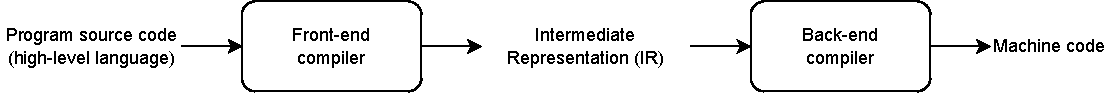
\includegraphics[width=\columnwidth]{figures/compiler/frontend-backend.pdf}
    \caption{Schematic of high-level steps in compilers that use \acf{IR}s. A source language-specific front-end compiler translates the source code into the \ac{IR}. There may be different front-end compilers for different source code languages, all translating to the same \ac{IR}. A machine code-specific back-end compiler translates the \ac{IR} to machine code. There may be different back-end compilers for different machine code types (i.e. targets). Optimizations may be applied on the \ac{IR}, or during front-end and/or back-end translation. This model allows flexibility: making a new source code language compatible only requires developing a new front-end compiler; making a new machine target compatible only requires a new back-end compiler. Furthermore, optimizations on the \ac{IR} code do not need to know about source code language nor target machine code.}
    \label{compiler:fig:frontend-backend}
\end{figure}

Compilers for classical computers perform code optimizations.
Code optimization techniques include
\begin{itemize}
  \item \emph{Target-independent optimization}, such as including removal of dead (unused) code, optimizations of looping constructs and combining common expressions to reduce code, and
  \item \emph{Target-dependent optimization}, such as register allocation, instruction re-ordering, branch prediction and elimination, vectorization and cache optimization.
\end{itemize}
These optimizations typically aim to improve execution speed and memory efficiency~\cite{aho_compilers_2006}.

\subsection{Compilers for classical networking.}
Classical applications that use networking are also compiled by classical compilers.
Typically, compilers do not apply network-specific optimizations.
This is since network operations are often handled by system calls, which compilers do not have control over.
Moreover, compilers also don't have control over the execution and timing of other applications in the network, nor over the network itself.
Network-specific optimization is therefore indirect, namely by optimizing the number of network system calls, reducing memory that would need to be context-switched upon network events, and optimizing local code that affects networking code~\cite{danalis_mpi-aware_2009}.
We note that there exist compilers for network programming languages~\cite{monsanto_compiler_2012, li_modular_2020}.
However, these relate to programming the control plane of networks (a paradigm called software-defined networking (SDN)), including how data is routed through the network, and are hence different from user applications that `merely use` the network.


\subsection{Compilers for quantum computing.}
\label{compiler:sec:compilers-qc}
As already described in \cref{chp:background}, quantum computing programs are typically expressed as quantum circuits.
Circuits consist of qubits, which are memory locations on which operations are applied.
Limit classical control may be added.

There exist many languages for quantum computing~\cite{chong_programming_2017, heim_quantum_2020}.
Many frameworks make use of assembly-like languages like OpenQASM~\cite{cross_open_2017} or cQASM~\cite{khammassi_cqasm_2018}.
Also more high-level languages exist such as Q\# and Scaffold~\cite{svore_q_2018, litteken_updated_2020, heim_quantum_2020}.

\paragraph{Circuit optimizers}
Compilers for quantum computing programs often try to optimize circuit depth (number of gates) and width (number of qubits).
Most compilers focus on \ac{NISQ} computers, dealing with resource constraints (like limited qubit availability, and restricted topology)\cite{chong_programming_2017, murali_full-stack_2019, bandic_full-stack_2022} and qubit mapping\cite{li_tackling_2019, zhang_context-sensitive_2020, bandic_mapping_2023, nishio_extracting_2020}.
Benchmarks exist with which to compare compilers, by looking at the output, like circuit size.

\paragraph{Hybrid classical-quantum compilers}
In the last years, more focus has been brought on hybrid classical-quantum compilers.
This can be seen in the proposal of full-stack architectures, including classical and quantum processing\cite{murali_full-stack_2019, khammassi_openql_2021, mccaskey_xacc_2020}, and the focus on hybrid quantum computing programs, like \acf{VQE}~\cite{diadamo2021distributed, liu2022layer} or \acf{QAOA}~\cite{farhi2014quantum}

One can distinguish two approaches:
\begin{itemize}
\item integration of classical and quantum code but optimization is separate or limited: \cite{litteken_updated_2020, fux_quingo_2021, khalate_llvm-based_2022, younis_quantum_2022}
\item joint classical-quantum optimization (MLIR-based, LLVM based): \cite{mccaskey_mlir_2021, ittah_enabling_2022, nguyen_retargetable_2022, peduri_qssa_2022}.
\end{itemize}

In order to deal with the hybrid code of hybrid programs, often intermediate representations (IRs) are used \cite{nigam_compiler_2021, nishio_inquir_2023}.
The existing LLVM framework has been re-used and integrated in quantum compilers \cite{murali_noise-adaptive_2019, murali_full-stack_2019, litteken_updated_2020}.
A quantum-specific IR has been created: QIR~\cite{haner_software_2018, geller_introducing_2020}.

% Qunity: formal hybrid language, but only compiles to circuit (openqasm).


% \cite{smith_error_2021} Mitigates decoherence by clever instruction ordering.
% Idea of going beyond layered model and ISA (e.g. directly pulse optimization): \cite{shi_resource-efficient_2020}.


% \begin{itemize}
% \item Catalyst (Xanadu Pennylane)
% \item QSSA compiles down to OpenQASM, which itself does not map to physical (virtual) qubits. In OpenQASM, you declare qubit registers, but the mapping to physical qubits only happens at runtime.
% \item Quantum Dialect (McCaskey/Nguyen) compiles to QIR, which also only contains the opaque `allocate`.
% \item QIRO does not explain how to lower it to native quantum instructions
% \end{itemize}

\subsection{Compilers for quantum networking.}
For quantum networking, compilation has not much been studied.
For distributed quantum computing, which is similar, compilers do exist~\cite{ferrari_compiler_2021, chatterjee_qurzon_2022, cuomo_optimized_2023, ferrari_modular_2023}.
One approach is to take the input circuit and first split it into separate circuits: circuit cutting~\cite{chatterjee_qurzon_2022}

Intermediate representations have also been proposed for network-related quantum programs:
an extension to QIR for network-related programs, NetQIR, has been proposed~\cite{vazquez-perez_netqir_2024}, and InQuIR~\cite{nishio_inquir_2023} for distributed quantum computing.


\subsection{Session types}
\label{compiler:sec:session-types}

Session types is a formalism used for defining communication protocols between different parties \cite{honda_language_1998}.
They can be used to for example specify the order in which messages need to be sent and received.
By having the protocol in a well-defined format, the parties can check whether they adhere to the agreed upon protocol.
Tools exist that can check at compile-time if a program adheres to a communication protocol~\cite{davidson_model_nodate, ardeshir-larijani_automated_2018}.
Session types may be used for two parties, but multi-party session types also exist \cite{honda_multiparty_2016}.
Multiparty session types have been considered for quantum network programs: \cite{lanese_towards_2024}.
Timed session types are an extension to session types, adding explicit time constraints to operations~\cite{bartoletti_timed_2017}.
Timed session types have not yet been applied to quantum.


\section{Design considerations}
\label{compiler:sec:design-considerations}
In this section we go through considerations to take into account when designing a compiler for Qoala programs.
In general, we want to re-use existing compilation strategies, but also need to address the unique challenges for compiling quantum network programs, as well as using features from Qoala like the hybrid representation and deadlines.
For optimization, the metrics we are interested in are makespan and application success probability.

\paragraph{Program elements}
Quantum network programs consist of four types of code: classical local (CL), classical communication (CC), quantum local (QL), and quantum communication (QC).
For purely CL and QL segments in the source code, existing compilation techniques can be used as described in \cref{compiler:sec:related-work}.

\paragraph{Hybrid classical-quantum code}
A compiler should take advantage of the fact that the Qoala executable contains both classical and quantum code.
This enables the compiler to perform optimizations on the mixed classical-quantum segments of the source code.


\paragraph{Networking operations}
Network operations (i.e. classical communication and entanglement generation) are slow compared to local operations.
For example, waiting to receive a classical message can take in the order of milliseconds (see \cref{fig:fig2}).
Also, entanglement generation may take milliseconds (\cref{fig:delcomp-epr-rate}).
By contrast, individual local quantum operations like gates take only microseconds (\cref{tab:gate_durations}) and local classical operations can be as fast as nanoseconds.
As can be seen in \cref{tab:exp_durations}, most of the time is spent on network processing.

Since quantum memory decoheres over time, a general optimization for the compiler is to minimize the time that quantum memory must remain idle during some other operation.
Because of the comparably long duration of network operations, special attention must be made by the compiler to minimize the time that there is quantum memory alive while doing a network operations.
This may mean that the compiler should re-order operations (without changing the behavior of the program) around network operations, such as exemplified in \cref{compiler:lst:reorder-network-ops}.

\paragraph{Non-deterministic times}
Not only are network-related operations slow, their duration is also non-deterministic (\cref{fig:delcomp-latencies-variance} and \cref{fig:delcomp-epr-rate}).
Even with optimizations (like re-ordering local operations) to minimize the time that quantum memory must remain alive, an network operation (such as entanglement generation) may take too long --- resulting in a too low quantum memory to produce meaningful results.
This raises two points:
(1) the compiler can use Qoala's feature of \emph{deadlines}: by adding (relative) deadlines to (parts of) the code, the compiler can hint to the scheduler to, at runtime, either abort the program or to retry a certain piece of code
(2) the question is what deadline the compiler should insert. For this, it may be possible for the developer to insert fidelity constraints in the high-level language (or as a compiler flag), such that the compiler can insert the corresponding deadlines (possibly parametrized by hardware characteristics from the \acf{EHI}, see \cref{qoala:sec:runtime_environment}).

\paragraph{Correctness guarantee of compiler}
A compiler must at all times guarantee that the behavior of the program does not change due to optimizations or rewrites.
For quantum network programs, this also means that any communication operations (classical communication of entanglement generation) must not be re-ordered among themselves.
This is because programs on other nodes in the network may expect these operations to happen in a certain order, and they cannot know of any re-orderings on this side.

\paragraph{Runtime performance depends on scheduler}
The compiler only affects the contents of the Qoala executable.
How well the program does at runtime also depends on (as shown in \cref{qoala:sec:evaluation})
(1) the network schedule, and (2) the node scheduler, especially in the case of multitasking (i.e. when other programs are executed concurrently with this program).
Specifically, this runtime scheduler affect both the makespan (time it takes to execute the whole program) and the average application success probability (see \cref{chp:background} for metrics).

\paragraph{Private program in networked context}
Recall that Qoala programs are part of multi-node applications, but that the compiler individually compiles the programs for a single node.
This means that program code must be compatible with code in the programs that are to be run on other nodes.
These other programs may not be in control by the developer nor the compiler.
For example, in a client-server application like BQC, a server node may already have implemented the server-side program, and advertises a service for clients to connect with, by describing a protocol that a client program should adhere to.
On the client side, a developer may write the client-side program.
This client program must be compatible with the server-side program, including the correct order of communication operations (both classical communication and entanglement generation operations), which may also include retries.
We may consider two alternatives:
\begin{itemize}
  \item It is the developer's responsibility to make sure the client program contains the correct order of communication operations, and hence adheres to the protocol.
  In this case, the compiler does not specifically know about the protocol; it will just optimize the program, and makes sure it does not re-order the internal ordering of communication operations (see consideration above).
  However, if the developer wrote the program in such a way that the program is not fully adherent to the protocol, the compiler cannot correct for this.
  \item There is a formal specification of the protocol, for example in the form of session types (\cref{compiler:sec:session-types}), which the compiler has access to.
  The developer must still make sure the program code adheres to the specification, but the compiler can perform an additional correctness check by evaluating protocol adherence, and warn the developer if this is not the case.
  If the protocol specification contains requirements about fidelity or timing, the compiler can, on top of checking for correctness, also try to meet these requirements by performing appropriate optimizations and inserting deadlines to guide the scheduler.
\end{itemize}



\paragraph{Target-specific optimization}
The compiler may perform optimizations specific to the hardware that a program will run on.
The \acf{EHI} (\cref{qoala:sec:runtime_environment}) can serve as the target for a compiler.



\section{Architecture recommendations}
We list recommendations for an architecture of a Qoala program compiler, based on the considerations above.

\begin{figure}[t]
    \centering
    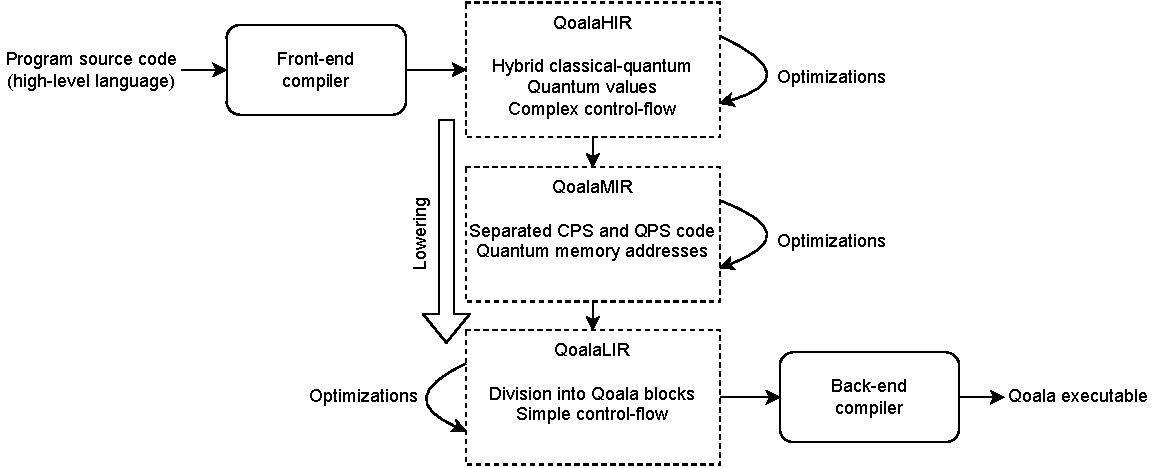
\includegraphics[width=\columnwidth]{figures/compiler/overall-design.pdf}
    \caption{Schematic of a high-level architecture for a Qoala program compiler.
    Overall, the same structure is used as in \cref{compiler:fig:frontend-backend}, but now with two \ac{IR}s.
    Source code (in any high-level language) is first translated into a high-level \ac{IR} called QoalaHIR. In this \ac{IR}, classical and quantum code can be mixed arbitrarily, allowing optimizations to be applied on the whole hybrid code.
    QoalaHIR has quantum values as native types, which enables the compiler to do (quantum) data-flow analysis in order to apply existing optimizations that make use of these def-use chains of quantum values~\cite{peduri_qssa_2022}. Control-flow may be complex.
    After applying optimizations on QoalaHIR, the program is translated to a low-level \ac{IR} (QoalaLIR) in which an explicit distinction is made between code that will run on the CPS and code that will be run on the QPS.
    Quantum values are now represented as pointers to memory locations, which means that quantum operations are in the circuit model, enabling existing quantum circuit optimization techniques.
    These optimizations may be hardware-specific and noise-aware.
    Finally, a back-end compiler translates the QoalaLIR code into Qoala program code.
    }
    \label{compiler:fig:overall-design}
\end{figure}

\subsection{Translation from high-level to Qoala}
\label{compiler:sec:translation}

\paragraph{Decouple front-end language from compilation framework by using Intermediate Representations (IRs)}

As explained in \cref{compiler:sec:related-work}, classical compilers typically use a hierarchy of steps: a front-end for any high-level language to an \acf{IR}, and a back-end for \ac{IR} to machine code.
Using an \ac{IR} decouples the main compiler design from specific input and output formats, making it more flexible and scalable.
Furthermore, if an \ac{IR} would be used that is already part of existing compilation frameworks, it can re-use existing compiler techniques.
The Quantum Intermediate Representation (QIR)~\cite{haner_software_2018, geller_introducing_2020} may be used.
However, QIR uses opaque pointers for quantum types, which prevents certain optimizations~\cite{ittah_enabling_2022, peduri_qssa_2022}.
\acf{MLIR} avoids these issues, since it allows for creating domain-specific \emph{dialects}.
Dialects have been created for quantum such that quantum types can be represented natively, allowing optimizations to be applied on operations including quantum ones~\cite{ittah_enabling_2022, peduri_qssa_2022}.
\cite{mccaskey_mlir_2021, nguyen_retargetable_2022} also use \ac{MLIR} before then compiling to QIR.

The front-end language is not a primary concern; we want to leave design and implementations open.
We also want to allow multiple (existing) high-level formats.
We recommend using the existing technique of IRs, gradually lowering code and performing optimizations at each level.
Specifically, we recommend \ac{MLIR} since it enables defining intermediate representations specifically for quantum networking, while still having access to standard (classical) LLVM optimizations.

One may consider at least two \ac{IR}s (\cref{compiler:fig:overall-design}):
\begin{itemize}
  \item A high-level \ac{IR} (QoalaHIR), consisting of a uniform hybrid classical-quantum representation of operations, where quantum values are native types.
  Native quantum values allow \emph{value-semantics}, meaning that quantum operations consume and produce quantum state values.
  This is in contrast with memory semantics where qubits are seen as pointers (such as in QIR~\cite{haner_software_2018, geller_introducing_2020}) and where quantum operations have side-effects.
  By using value-semantics, the compiler can perform (quantum) data-flow analysis in order to apply classical optimization techniques such as loop unrolling or dead code elimination~\cite{peduri_qssa_2022, ittah_enabling_2022}.
  \item A low-level \ac{IR} (QoalaLIR), where classical code is explicitly separated from quantum code.
  The classical code segments will eventually compile down to classical Qoala blocks (classical local and classical networking blocks, \cref{qoala:sec:program_structure}), while quantum code segments will eventually compile down to quantum Qoala blocks (local routines and request routines, \cref{qoala:sec:program_structure}).
  The explicit separation (1) makes it easier to perform the back-end compilation step (going from low-level IR to Qoala executable) since the formats are already similar and (2) forces the compiler to decide on \emph{where} to make the separations, allowing it to optimize it (see below).
  QoalaLIR explicitly maps qubit values to quantum memory locations, hence not using value-semantics.
  By including quantum memory, the compiler can do hardware-specific optimizations such as qubit mapping.
\end{itemize}


\paragraph{Support fidelity and timing constraints in high-level language}
As mentioned above, we do not want to specify one specific high-level language for developers to write their quantum network programs in.
Instead we want to allow multiple (existing) high-level formats in order to provide flexibility in adoption.
The NetQASM SDK (\cref{chp:netqasm} and \cref{chp:qnodeos}) may be used.
However, we recommend adding constructs to the high-level language for supplying fidelity and timing constraints.
In this way, the developer can indicate that certain parts of the code are critical, and that the compiler should handle this by adding deadline constraints.
For example, a developer may indicate that a particular qubit variable must have at least $F$ fidelity compared to some ideal state at the moment it gets measured;
the compiler, seeing that certain network-related operations happen while this qubit is alive, may estimate the fidelity of the qubit as a function of how long these operations take.
In order to meet the required fidelity, then, the compiler can insert a deadline for the network-related operations corresponding to the maximum time that still realizes fidelity $F$.


\paragraph{Use EHI as compilation target}
A compiler must have an explicit \emph{target} that describes the software and hardware characteristics that the compiled executable must be compatible with.
This target includes at least the qubit topology of the quantum memory and the NetQASM flavor (i.e. the allowed quantum instructions, see also \cref{netqasm:sec:design_decisions_language}).
This information can come from the \ac{EHI}.
We note that the \ac{EHI} also contains information about noise and durations (of gates and network operations).
This information may or may not be used by the compiler for optional optimization, but is not part of the target.

\paragraph{Optionally use session types for protocol adherence checking}
As mentioned in \cref{compiler:sec:design-considerations}, a program typically implements some multi-node protocol that has certain requirements on communication order and possibly fidelity or timing.
If such a protocol would have a formal description in the form of session types, a compiler for Qoala programs should check the program's contents and see if it adheres to the protocol.

\subsection{Optimization}
The compiler should optimize programs with respect to various metrics.
Some of these metrics are those from standard compilers: memory usage and execution time (or makespan).
This holds for both classical and quantum code.
For classical code, existing optimization can be used from MLIR (part of LLVM), applied on the program when it is in QoalaHIR or QoalaLIR (\cref{compiler:fig:overall-design}).
For quantum code, also existing techniques can be used, see \cref{compiler:sec:compilers-qc}.
These include circuit mapping and gate optimization techniques.

Moreover, by using the hybrid classical-quantum format of QoalaHIR we can re-use existing optimizations such as loop unrolling and other, see \cite{mccaskey_mlir_2021, ittah_enabling_2022, nguyen_retargetable_2022, peduri_qssa_2022}.
This also enables cross-subroutine optimizations, something not possible in NetQASM.

Other metrics the compiler should optimize for are
\begin{inlinelist}
\item Amount of CPS-QPS communication, since this negatively impacts execution time and possibly the time that quantum states must remain in memory,
\item Success probability of the application. In general this is application specific, but a good heuristic is to reduce the time that quantum states remain in memory, which may be done by adding deadlines that help the scheduler.
\end{inlinelist}

As with classical network or internet applications, the performance of quantum network applications also depends on the network itself, on which the compiler does not have influence.
A large factor in performance is the fidelity (quality) of entangled states produced by the network.
Although the compiler does not control this fidelity directly, it can indirectly help by doing clever capability negotiation (see also below) and adding deadlines.

Furthermore, the compiler should do noise-aware optimization including existing techniques for local quantum operations~\cite{smith_error_2021, murali_noise-adaptive_2019}.


\textbf{Re-use existing (classical and quantum) compilation techniques for local code}
These include classical techniques like loop unrolling, and quantum techniques (qubit mapping, gate optimization, see \cref{compiler:sec:related-work})
Existing quantum circuit optimizations can be applied to local quantum code in the quantum network program to compile.
For network-related operations, see below.

\textbf{Perform optimizations on joint classical-quantum representation}
Make use of the fact that classical and quantum code can be jointly analyzed and optimized.
Use existing techniques, see \cite{mccaskey_mlir_2021, ittah_enabling_2022, nguyen_retargetable_2022, peduri_qssa_2022}.
Use existing \ac{MLIR} infrastructure.

\textbf{Optimize using noise characteristics}
As mentioned above, the compiler's target comes from the \ac{EHI}, which contains information about noise and durations (of gates and network operations).
The compiler can use this information to do specific optimizations, including
\begin{itemize}
  \item Compiling to specific NetQASM flavor
  \item Mapping to specific qubits with better topology
  \item Noise-aware optimizations such as~\cite{smith_error_2021, murali_noise-adaptive_2019}
\end{itemize}


\textbf{Give hints to scheduler (deadlines)}
In \cref{compiler:sec:design-considerations} we mentions that the compiler could add deadlines for parts of the code in order to meet fidelity requirements that are put in the code by a developer or that may come from a protocol description.
The compiler may do so by analyzing the code and estimating the fidelity of certain quantum memory at a given moment in time, as a function of the time it took to do the operations before.
It can use the \ac{EHI} for this, which contains information about gate duration, estimated network operation duration, and coherence times of qubits.
For this, algorithms would need to be developed to perform the estimation.
The deadline can then be used by a scheduler, and depending on the scheduling algorithm, these may increase the application success probability.

\textbf{Do network-specific optimizations}
On top of the existing optimizations for classical and quantum local code (mentioned above), the compiler should try to perform optimizations relating to networking operations, as mentioned in \cref{compiler:sec:design-considerations}:
\begin{itemize}
  \item Re-order operations to minimize qubit memory time (see \cref{compiler:lst:reorder-network-ops} for a simple example).
  % AFAIK not done in any other compiler (hybrid classical-quantum reordering yes, but not specifically to reduce qubit `live' time)
  \item Even without protocol description: do not re-order external operations.
  \item Add deadlines to code blocks to guide scheduling
\end{itemize}

\begin{figure}[t]
  \centering
  \begin{lstlisting}[language=Python]
q = init_local_qubit()
q.H()  # hadamard
e = create_epr()
q.H()  # hadamard
q.measure()
  \end{lstlisting}
  \caption{Simple program that (1) initializes a local qubit $q$, (2) applies a Hadamard gate on it, (3) creates an entangled qubit $e$, (4) applies another Hadamard gate on $q$ and (5) measures $q$.
  $q$ are completely independent in terms of application logic.
  Since the creation of the entangled qubit $e$ may take a long time, executing the operations in the order they are given means that $q$ ---after the first Hadamard --- must remain in memory while waiting for the entanglement generation too finish.
  During this time $q$ might decohere considerably.
  An optimization would be to move the entanglement creation to the very end (after measuring of $q$) such that the initialization, gates, and measurement of $q$ happen in one go, providing best performance.
  }
  \label{compiler:lst:reorder-network-ops}
\end{figure}


\section{Conclusion}
We have discussed design considerations for a Qoala program compiler, and proposed a high-level architecture for such a compiler.
Our overall recommendation is to re-use existing compilation techniques wherever possible, such as for purely classical code segments and purely local quantum code segments.
We also recommend using existing infrastructure such as MLIR in order to (1) re-use existing techniques and (2) represent the hybrid nature of quantum network programs.
Moreover, we have provided pointers for (quantum) network-specific optimizations, including instruction re-ordering and inserting deadlines to code blocks.

More research is needed for the ideas presented in this chapter before a detailed compiler design can be completed.
For example, how should developers describe their fidelity constraints in high-level source code?
How can a compiler translate such constraints into deadlines?
Also, the idea of using session types for protocol descriptions must be investigated more.
Finally, evaluation of the compiler design is crucial to test the merit of these ideas and to guide further research.
Evaluation may be done by inspecting the compilation output (for instance, the number of (blocks of) instructions in the Qoala executable) or the runtime performance.
However, we note that the runtime performance (including makespan and application success probability) also depends on the node scheduler and network schedule.
Therefore, future research may want to focus on the joint compilation-scheduling problem.
